\documentclass[10pt,a4paper,parskip=full]{scrartcl}
\usepackage[utf8]{inputenc}
\usepackage[T1]{fontenc}
\usepackage[english]{babel}
\usepackage[hidelinks]{hyperref}
\usepackage{tabularx}
\usepackage{dcolumn}
\usepackage{graphicx}
\usepackage{ragged2e}

\newcolumntype{Y}{>{\centering\arraybackslash}X}
\graphicspath{{./img/}}

\title{Compression method for multiple image compressing}
\author{David Nelles}
\date{16.07.2019}
\begin{document}
	\maketitle
	\newpage
	\tableofcontents
	\newpage
	\section{The idea}
	The idea is to create an average image of all images, that should be compressed. Afterwards the pixels, which differ especially from the average image are saved for each image.
	
	To be more exact, it is important to sort the images. It is not good, to create an average image of completely random images. There have to be similarities between the images, you create the average image from.
	
	\section{Theoretical problems}
	There are some problems with this method:
	
	This is a lossy compression method. The following problem coheres with that.
	
	If you want to add images to the compression, the average image will change. After a few times, it could be, that some pixels of the average image differ more than allowed. That is, because you do not want to save the whole image history. For example, if the pixel in the average image and a specific image is black, the pixel is not saved separately. It could be, that the average pixel turns to gray after adding some images to the compression. If this gray does not differ enough, from the specific image from before, it will still not be saved separately. If you add some further images, the pixel could turn to light gray. Light gray and black differ enough, that the black pixel would be saved separately. But it is not possible, to find out, which color the pixel had before. You only know, that this pixel is not saved separately. So you have to guess, that the color of the pixel is gray like the color of the same pixel in the average image. It could be, that this problem turns a pixel of an image into a completely new color.
	
	\section{Testing}
	The first step to test the method is to take images with similarities. This is done manually.
	
	To test this method, a program was written. The program creates an average image of all images of one similarity category. Afterwards the differences between the original images and the average image are determined.
	
	Therefore, the red, green and blue values of each pixel are compared. If one of these values differ more than a given percentage from the color of the average image pixel, the exact color of the original image is saved. Else the pixel color of the new image is set to transparent.
	
	To check how good the method work, you can take the average image and add a specific image as new layer above the average image. In the following there are some examples.
	\newpage
	
	\subsection{Lightning example}
	\centering Average image\\
	\includegraphics[width=\linewidth]{lightning_average}
	\newpage

	\centering Original image\\
	\includegraphics[width=\linewidth]{lightning_original}
	\begin{tabularx}{\linewidth}{Y|Y}
		compressed image & avarage in background\\ \hline
	
		\multicolumn{2}{c}{90\%}\\
		
		\includegraphics[width=\linewidth]{90/lightning_neg}
	 &
	 	\includegraphics[width=\linewidth]{90/lightning_result}\\ \hline
	 	
	 	\multicolumn{2}{c}{80\%}\\
	 	
	 			\includegraphics[width=\linewidth]{80/lightning_neg}
	 	&
	 	\includegraphics[width=\linewidth]{80/lightning_result}\\ \hline
	\end{tabularx}

	\subsection{Rabbit example}
	\centering Average image\\
	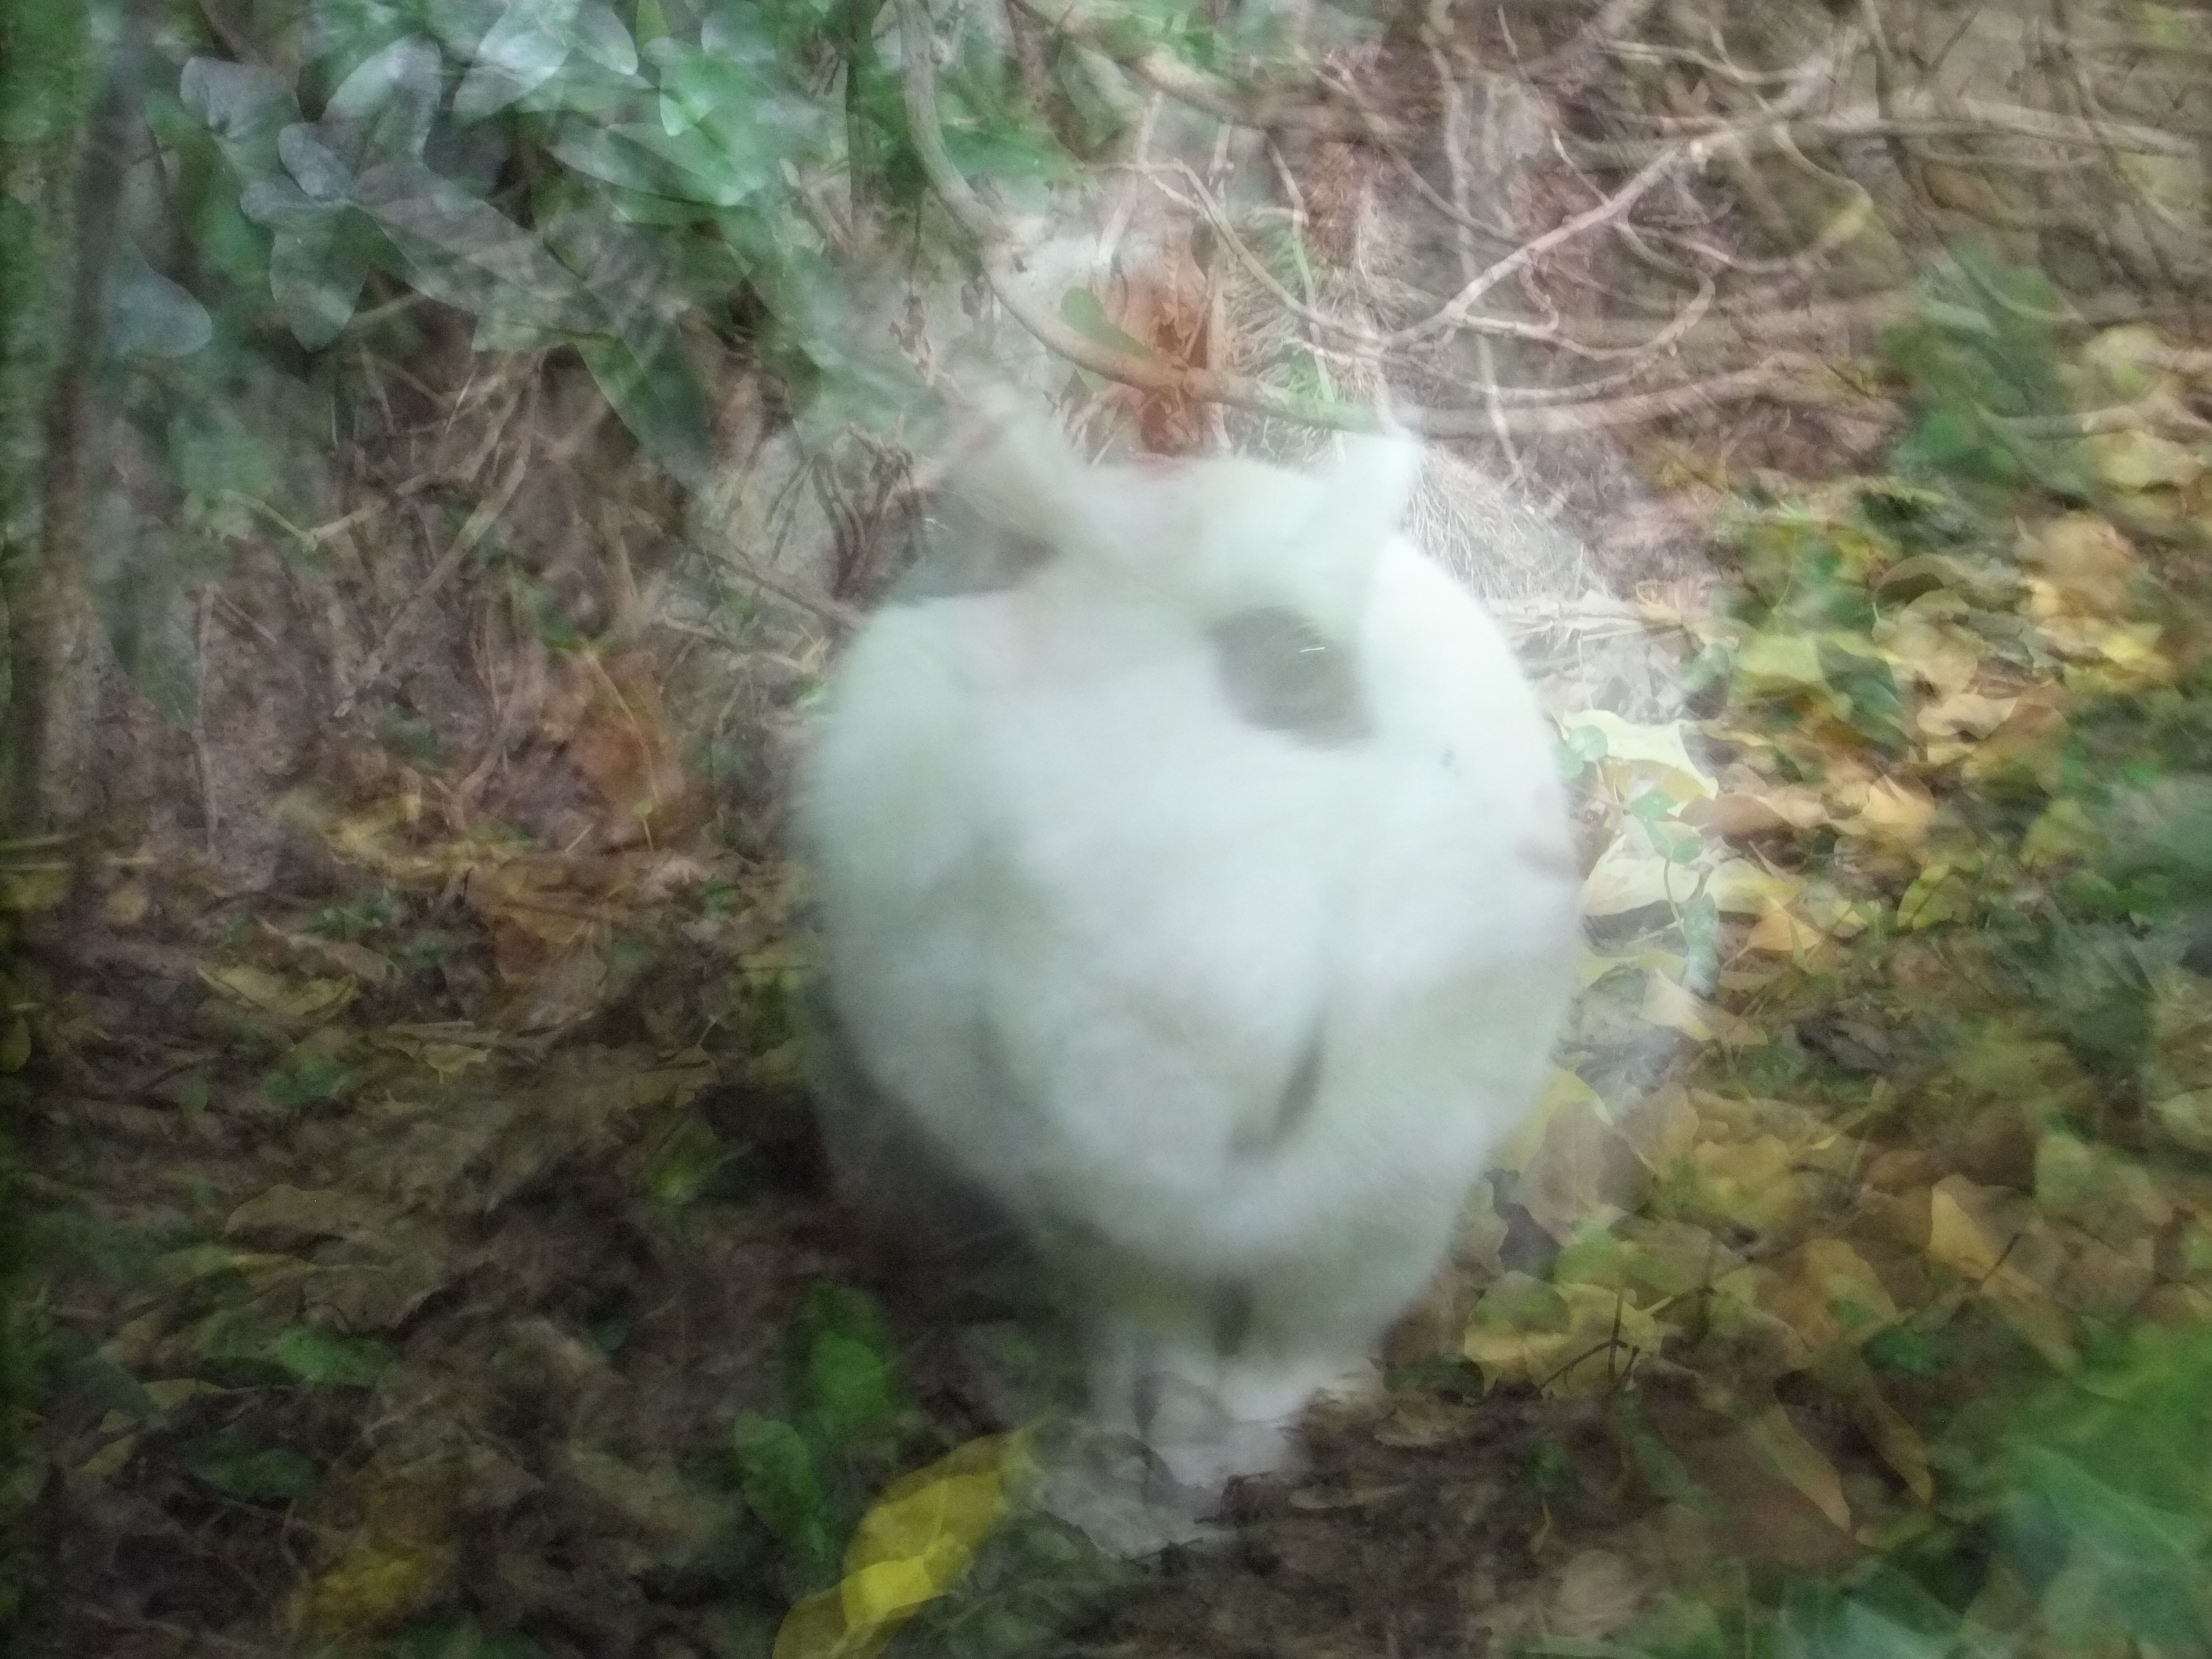
\includegraphics[width=\linewidth]{rabbit_average}
	\newpage

	\centering Original image\\
	\includegraphics[width=.88\linewidth]{rabbit_original}\\
	\begin{tabularx}{.88\linewidth}{Y|Y}
		compressed image & avarage in background\\ \hline
		
		\multicolumn{2}{c}{90\%}\\
		
		\includegraphics[width=\linewidth]{90/rabbit_neg}
		&
		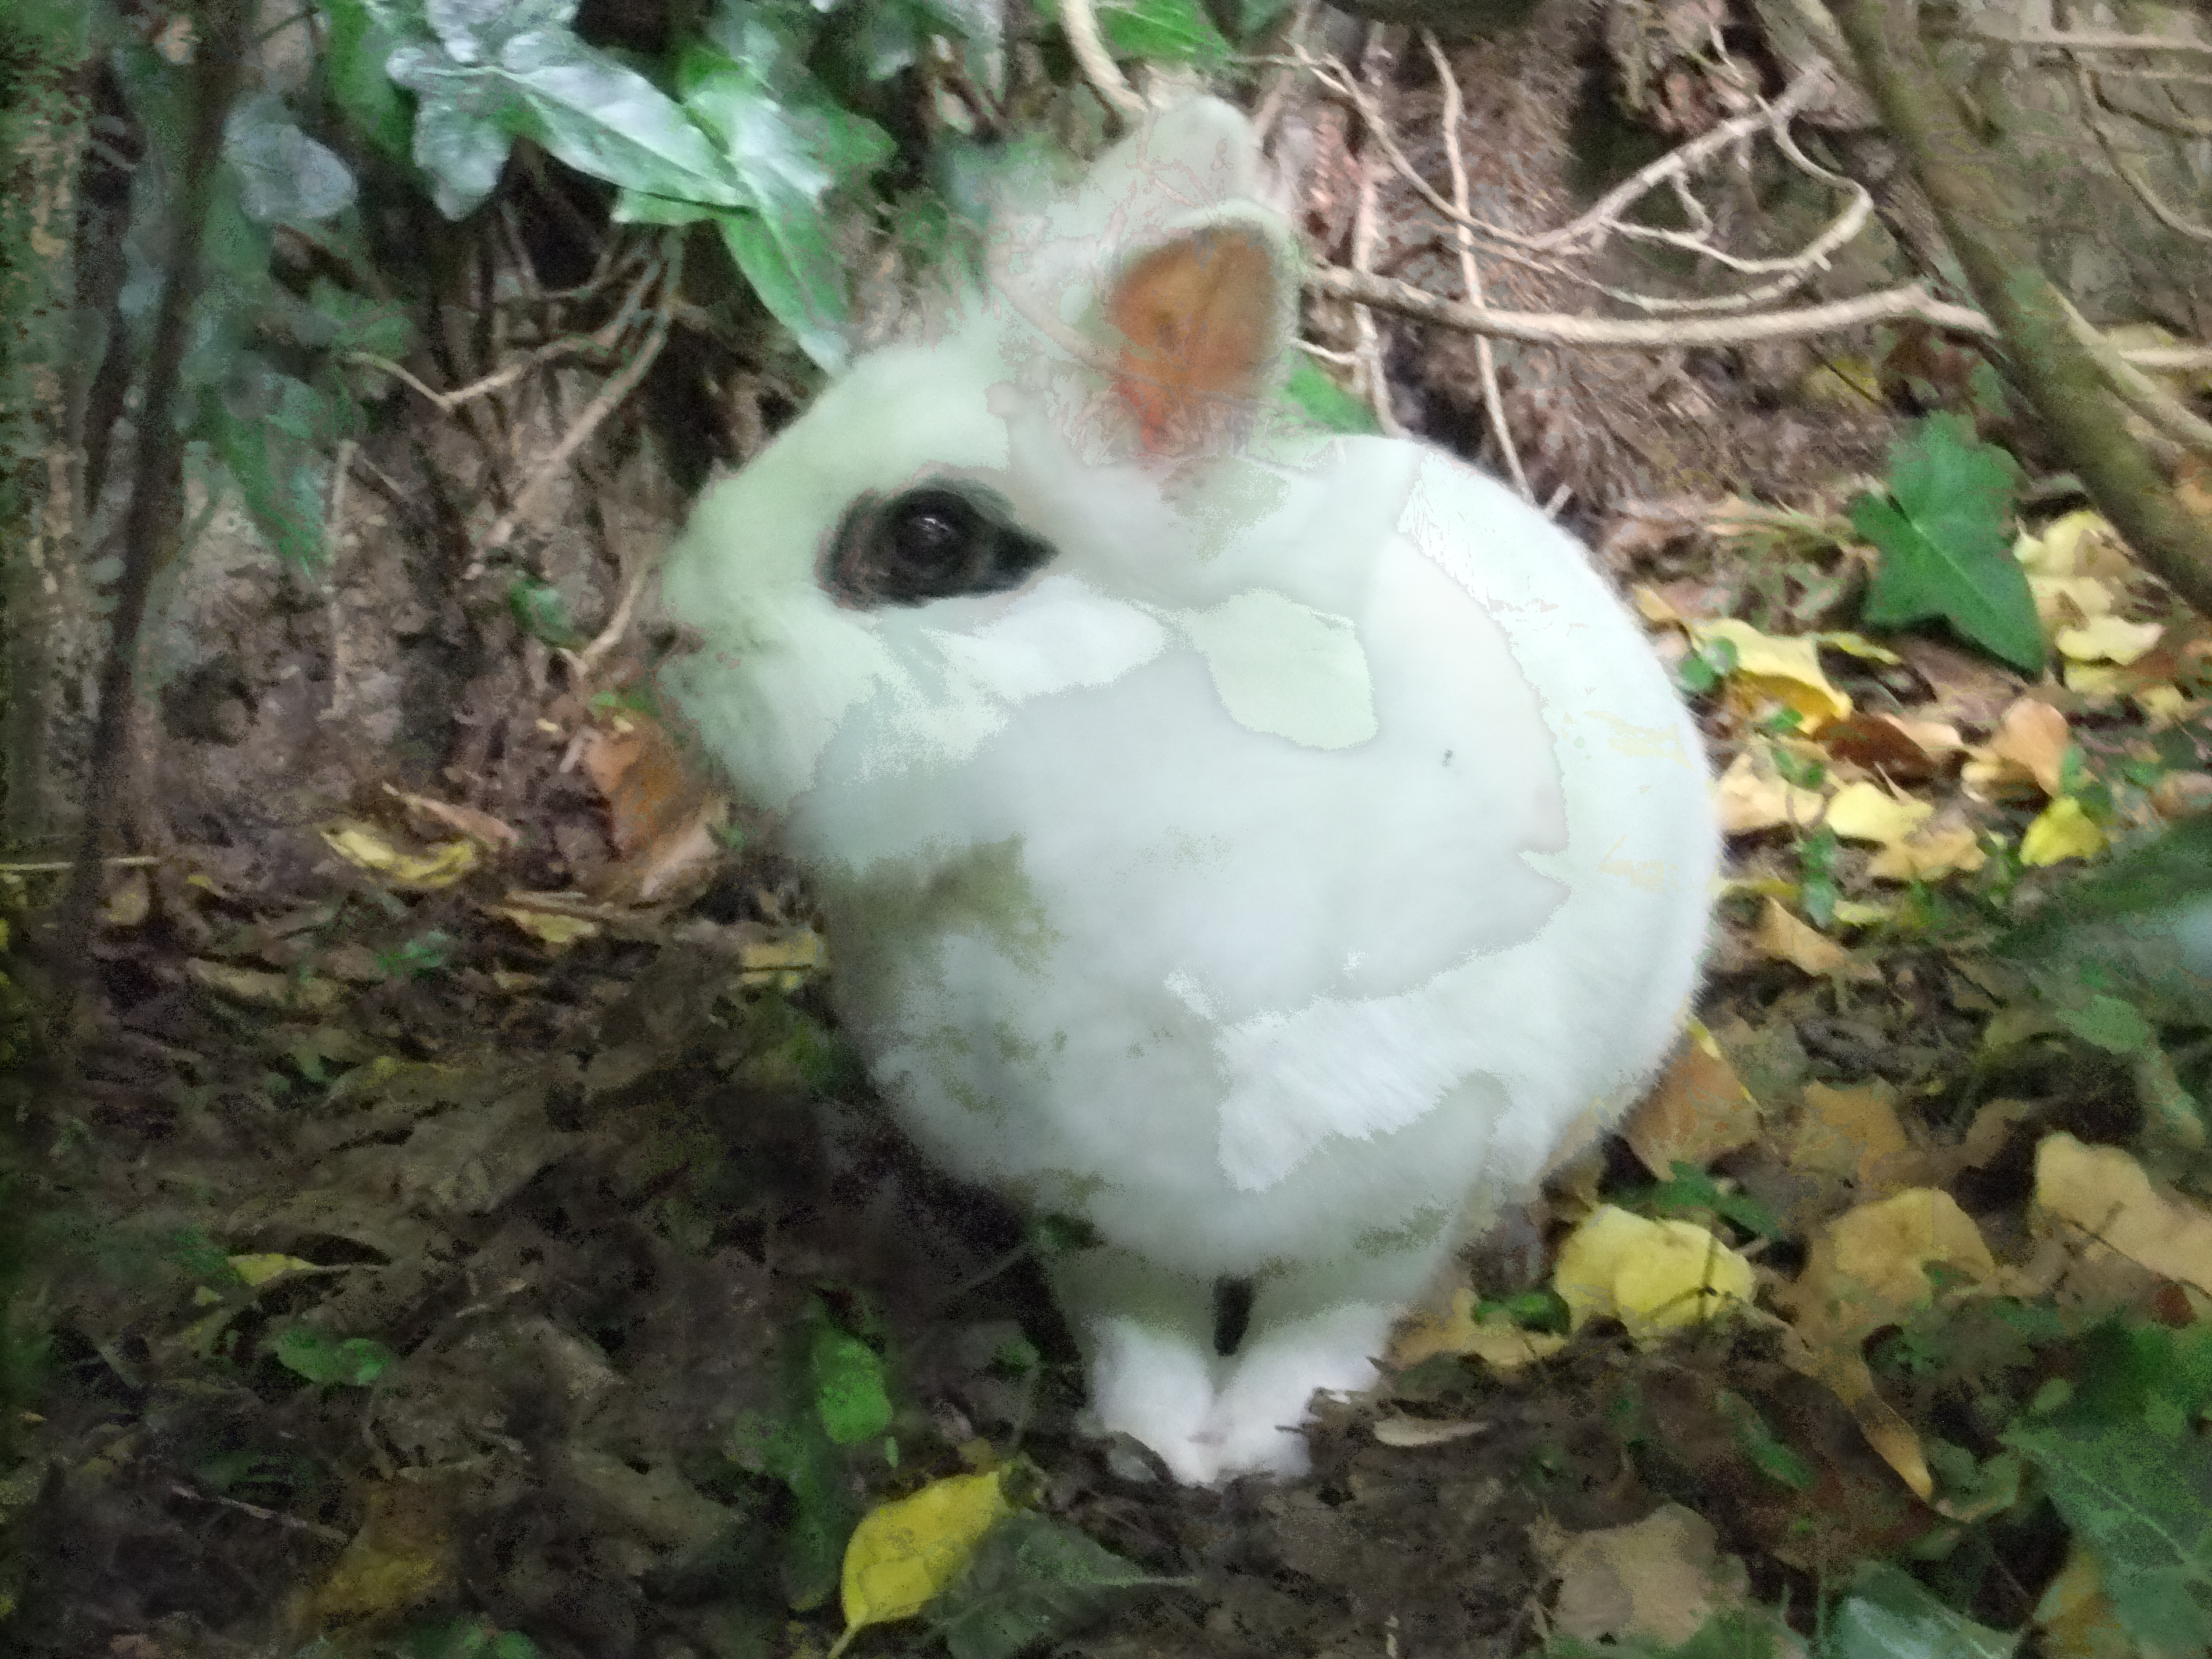
\includegraphics[width=\linewidth]{90/rabbit_result}\\ \hline
		
		\multicolumn{2}{c}{80\%}\\
		
		\includegraphics[width=\linewidth]{80/rabbit_neg}
		&
		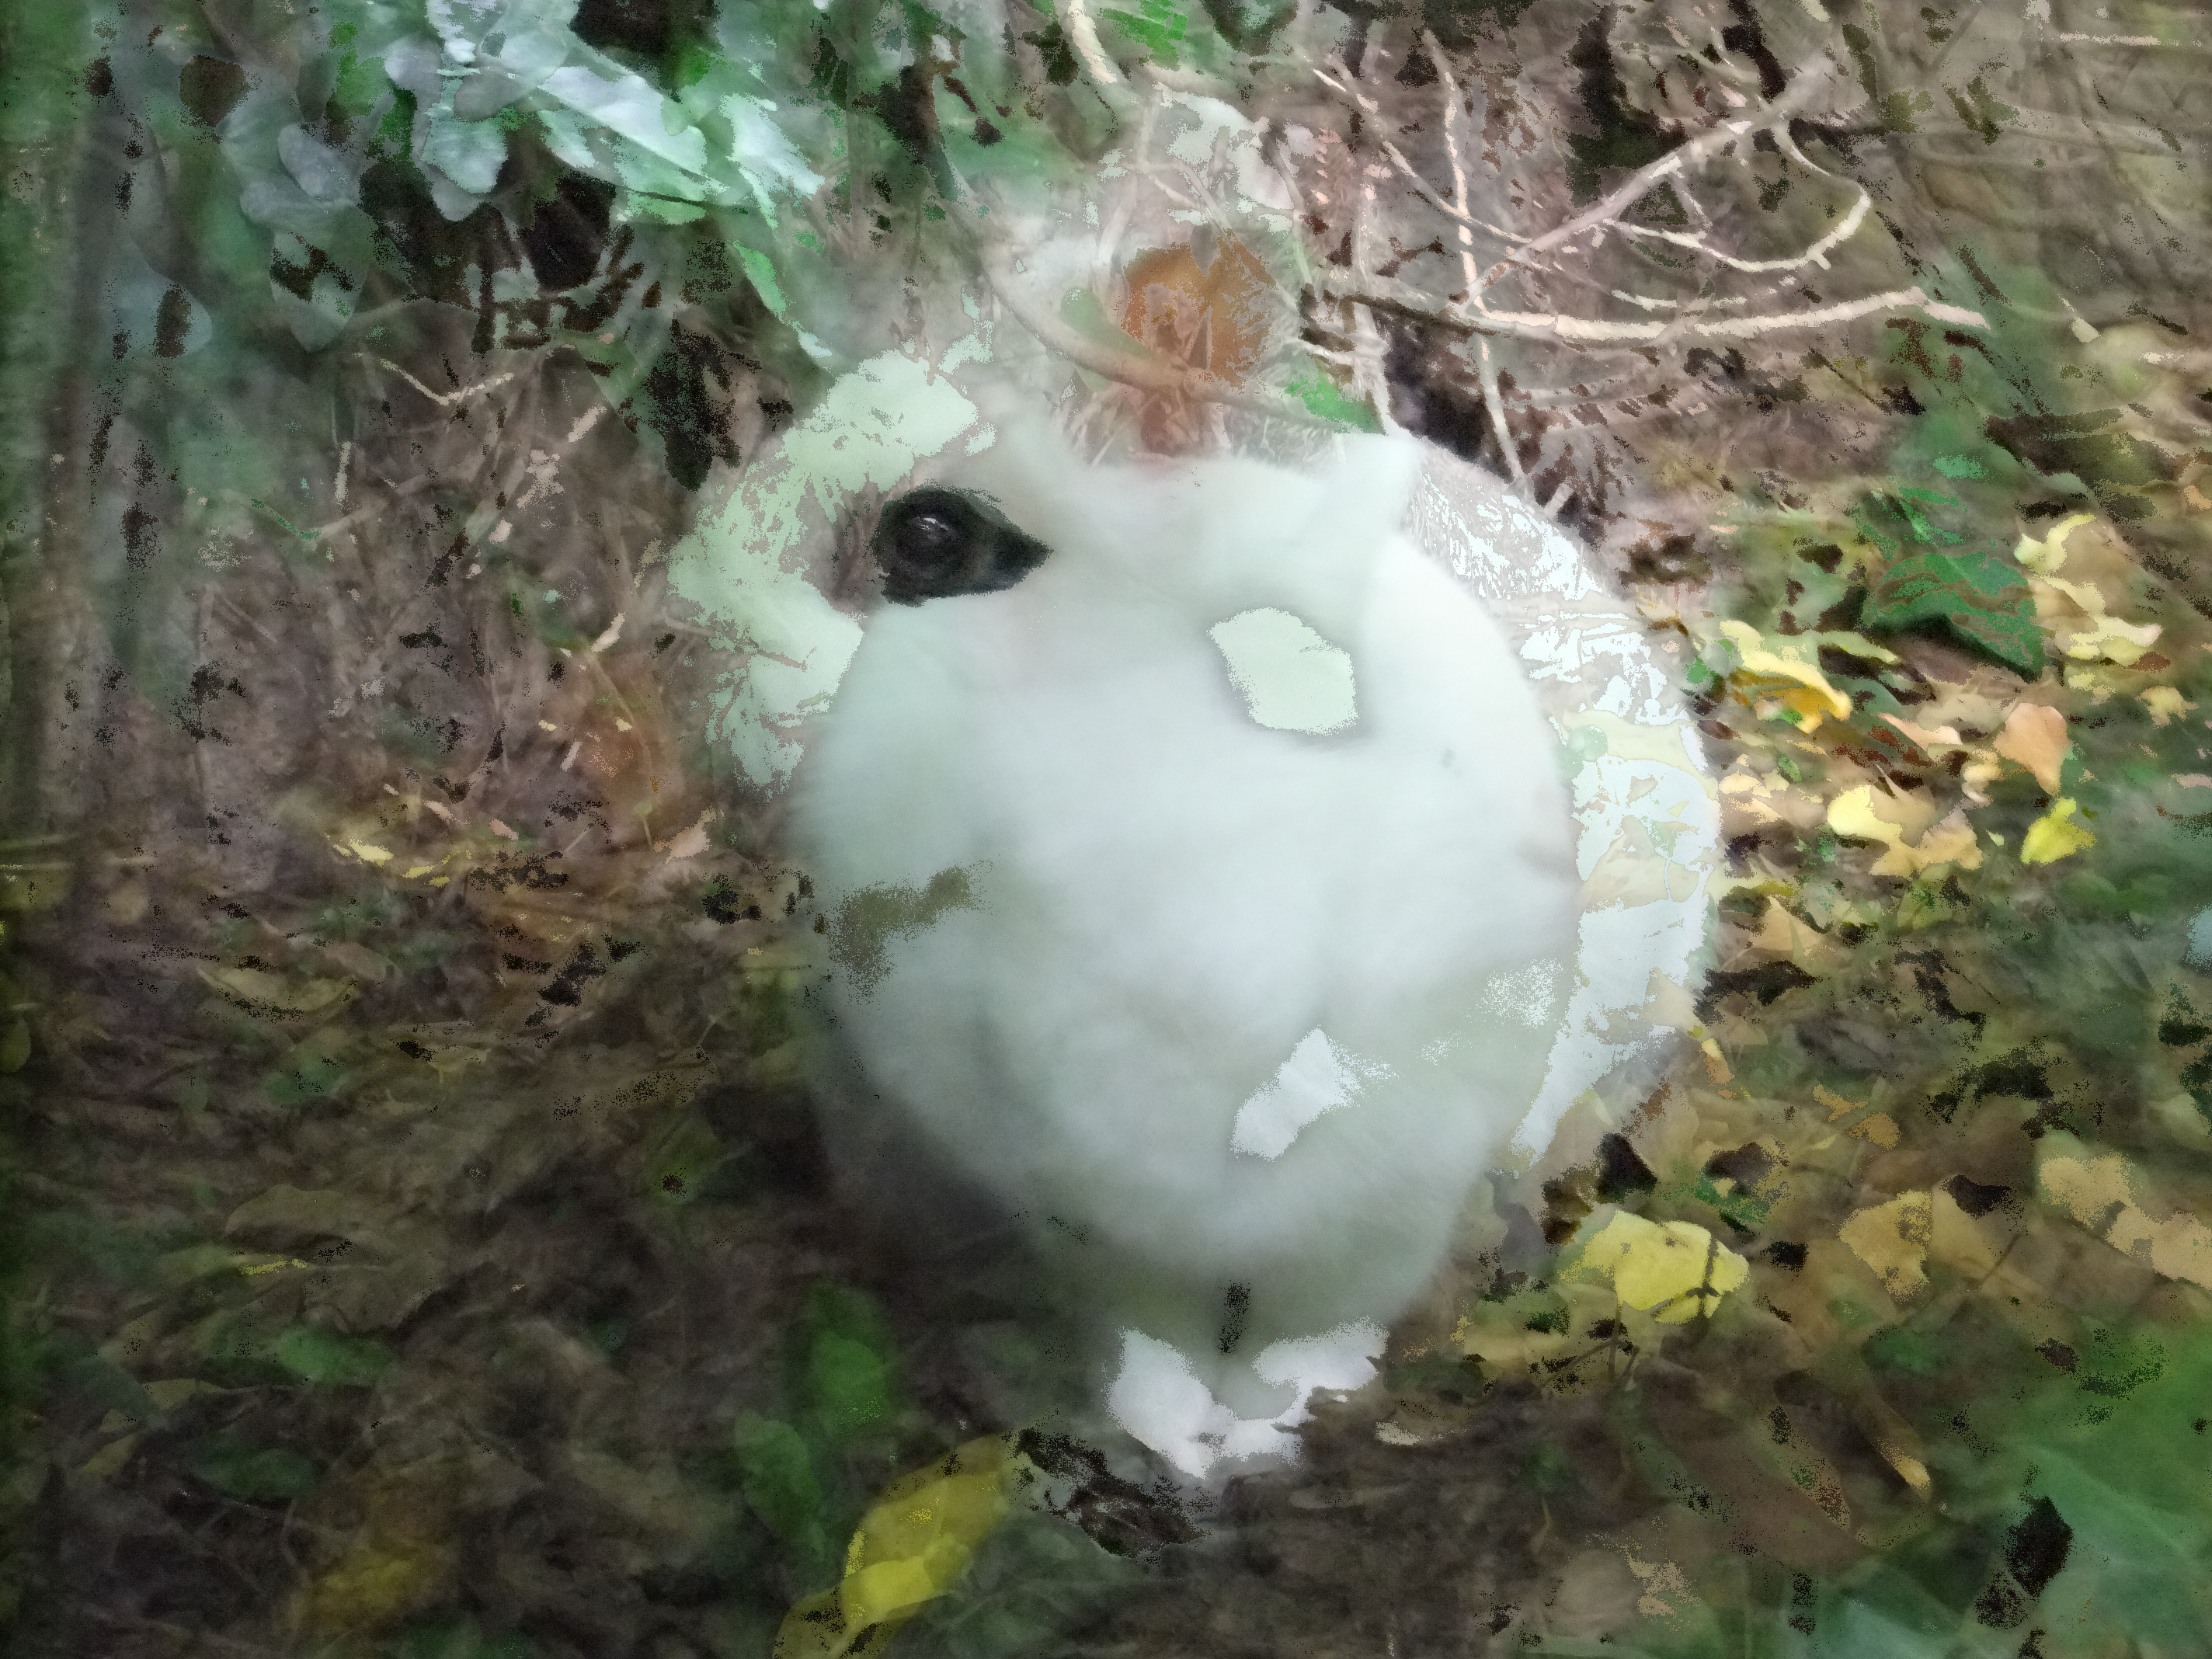
\includegraphics[width=\linewidth]{80/rabbit_result}\\ \hline
	\end{tabularx}

	\justifying

	\section{Practical problems}
	As you can see in the examples, there is the problem, that prominent objectives into images affect the average image more than other objectives. This prominent object has to be overwritten by every image, that do not have this object or where the object has another shape. Especially in similar images the prominent object has often nearly the same color as the color of the pixels around that object. Prominent objects are often the areas of an image, where the focus is. That means, that this object has to be very clear.
	Therefore, the percentage of accordance have to be very high. 80\% accordance is mostly not enough. There has to be 90\% accordance to reach an image where you can't see prominent objects multiple.
	
	Another problem is, that the border between the separate saved pixels and the pixels of the average image are very strict. Even with a high percentage of accordance this border is very unattractive.
	
	\section{Result}
	The compression method can only be used for images, you don't want to see in a high resolution. For example, for thumbnails. But it has to be chosen a high percentage of accordance. That means, that more pixels are saved separately. The result of that is, that more images are needed to get a good compression ratio.
\end{document}
